% !TeX spellcheck = ru_RU
% !TeX encoding = UTF-8
\chapter{Конформационное поведение производных и гетероаналогов бицикло[3.3.1]нонана (обзор литературы)}\label{ch:Review:Basics}

Конформационный анализ органических циклов скоро обязательно отметит какой-нибудь свой очередной юбилей, однако до сих пор он интересен, потому что полон неожиданностей и находит столь же неожиданные применения. Он находится где-то на пересечении физической, органической, структурной, математической химии, молекулярного моделирования, стереохимии\dots
Ставит целью изучение закономерностей и~прогнозирование различных свойств вещества, реакционной способности, биологической активности и~т.~п. в~зависимости от~качественных характеристик и~количественных параметров геометрического строения молекул этого вещества.

Закономерности строения шестичленных (в особенности "--- насыщенных) циклов хорошо изучены, а соответствующие исследования остаются краеугольным камнем конформационного анализа (здесь и~Нобелевская премия сэра Дерека Бартона, и~много подобного). Неаддитивность и~нелинейность в~поведении 1,2-конденсированных колец в молекулах производных \emph{цис}- и~\emph{транс}-декалинов (декагидронафталинов, бицикло[$4.4.0$]деканов), а~также 1,4-конденсированных (бицикло[$2.2.2$]октанов) широко известны и~весьма подробно изучены. Сравнительно с ними 1,3-конденсированные шестичленные циклы, образующие систему бицикло[3.3.1]нонана, выглядят малоизвестными и~загадочными в своём конформационном поведении.

\begin{center}
  \begin{tabular}{cc|cc}
\multicolumn{2}{c|} {\chemfig{[:-30]*6(-(-[:180]-[:120]?)----(-[:-180]?)-)} \chemfig{[:-30]7*6(-6-5(-[:0]4?[a])-9-1(-[:0]2-[:-60]3?[a])-8-)} %
% $\equiv$ \chemfig{[:-30]*6(--(<[:-90,0.75]H)(-[:0]?[a])--(<[:+90,0.75]H)(-[:0]-[:-60]?[a])--)} %
}
     &
    \chemfig{[:-30]*6(------)} &
    \\
    \multicolumn{2}{c|}{бицикло[$3.3.1$]нонан} &
    циклогексан &
    \\
    \multicolumn{2}{c|}{\cmpd{Bicycle331}} &
    \cmpd{Cyclohexane} &
    \\  \midrule
    \chemfig{*6(--(<[:-90,0.75]H)(*6(-----))-(<[:+90,0.75]H)----)} &
    \chemfig{*6(--(<[:-90,0.75]H)(*6(-----))-(<:[:+90,0.75]H)----)} &
    \chemfig{?[a]<[:-120]-[:+30,,,,line width=\boldbondwidth](-[:+90,,,,line width=\boldbondwidth]>[:+60]-[:-90](?[a])?[b])-[:-30,,,,line width=\boldbondwidth]>[:+60]?[b]} &
    \\
    \emph{цис}-декалин &
    \emph{транс}-декалин &
    бицикло[$2.2.2$]октан &
    \\
    \emph{цис}-{\cmpd{Decaline}} &
    \emph{транс}-{\cmpd{Decaline}} &
    \cmpd{Bicycle222} &
    \\
  \end{tabular}
\end{center}

Исследования конформационного поведения аналогов бицикло[$3.3.1$]\-нонана в целом обобщены примерно до~конца 1980-х годов~\cite{Zefirov:1991a}. В~последнее время появился ряд обзорных работ, охватывающих специальные свойства ряда производных систем, в основном биспидинов (3,7-диазабицикло[$3.3.1$]нонанов): их координационная химия~\cite{Comba:2007}; их~биологическая активность в~общем~\cite{Tomassoli:2016} и~применение для~радиотерапии~\cite{Comba:2018}. Эти свойства оказываются явным образом зависимыми от~предпочтительной конформации, принимаемой бициклическим скелетом молекулы.

\section{Предварительные замечания и соглашения о терминах и обозначениях}

\epigraph{Quia igitur huius mundi machina sphaerica est, dicendum est in primis quid sit sphaera?}{De sphaera Lincolniensem Secundum tractatus cap. I}

Терминология конформационного анализа не~считается устоявшейся и~поныне, поэтому нам показалось полезным, чтобы не~сказать "--- необходимым, с самого начала по~возможности прояснить дальнейшее словоупотребление. Здесь и~далее термины \tqt{\emph{форма молекулы}} и~\tqt{\emph{конформация}} в~сильной степени взаимозаменяемы и обозначают геометрическую структуру молекулы, тогда как обозначение \tqt{\emph{конформер}} говорит прежде всего о~конформации, которую принимает молекулярная структура, обладающая \emph{динамической устойчивостью}, то есть соответствующая минимуму на~\tqt{\emph{поверхности потенциальной энергии}} (ППЭ) данной молекулярной системы в рамках некоторой \tqt{\emph{модельной химии}} (согласованной совокупности экспериментальных, теоретических или~вычислительных методов, выбранных для~моделирования и~численной оценки свойств молекулярной системы посредством того или~иного приближённого расчёта её ППЭ).

Другим распространённым подходом к определению конформаций является рассмотрение конформационного перехода в молекуле как согласованного изменения определённой совокупности двугранных углов, мало затрагивающего длины связей и~валентные углы как более жёсткие энергетически структурные параметры\dots

Без специального доказательства или обоснования в дальнейшем принимается интуитивно понятное утверждение, что конформация всей молекулы однозначно определяется конформацией её \emph{остова}, подструктуры, состоящей из~неводородных атомов.
Под термином \tqt{\emph{циклическая система}} здесь и в дальнейшем мы подразумеваем молекулярные циклы и полициклические каркасы, рассматриваемые как часть молекулы, и~прежде всего "--- часть её остова, в~значительной степени влияющая на~итоговую конформацию всей молекулы.

В органической химии именно углеводороды являются опорными, референсными соединениями; отличие в свойствах их производных является результатом возмущения под действием введённых заместителей (Бутлеров и \tqt{химическое сродство}???). Здесь и~далее используется широкое понятие \tqt{замещения} в циклических системах. То есть, если не~оговаривается иное, под~этим термином рассматривается не~только введение или изменение заместителя (замещение в~более узком смысле), но~и~\emph{гетероаналогия} (или~\emph{гетероаналогичное замещение}) атома углерода соответствующего циклического углеводорода на~гетероатом того же стереохимического типа.

\begin{figure}
  \caption{Стереохимическая типизация атомов циклических систем\label{fig:Atom:Types}}

  \vspace{\bigskipamount}
  \centerfloat{
    \textbf{Двухкоординированные~(тип~I)}

    \ChemPicture{>[:+30]\circ-[:+150]}

    \begin{tabular}{c|}
%      \chemfig{>[:+30]B(-H)-[:+150]} &
      \chemfig{>[:+30]B(-R)-[:+150]}  \\
    \end{tabular}
    ~
    \begin{tabular}{cc|}
      \chemfig{>[:+30]C(-[:+60]R)(-[:-60]R{'})-[:+150]} &
      \chemfig{>[:+30]C(=[:0,0.875]X)-[:+150]} \\
    \end{tabular}
    ~
    \begin{tabular}{cc|}
      % \chemfig{>[:+30]N(-H)-[:+150]} &
      \chemfig{>[:+30]N(-R)-[:+150]} &
      \chemfig{>[:+30]N\rlap{${}^+$}(-[:+60]R)(-[:-60]R{'})-[:+150]}\\
\end{tabular}
~
\begin{tabular}{c|}
\chemfig{>[:+30]O-[:+150]} \\
\end{tabular}

    \begin{tabular}{c|cc|}
      \chemfig{>[:+30]Si(-[:+60]R)(-[:-60]R{'})-[:+150]} &
%      \chemfig{>[:+30]P(-H)-[:+150]} &
      \chemfig{>[:+30]P(-R)-[:+150]} & \chemfig{>[:+30]P(-[:+60]R)(=[:-60,0.875]O)-[:+150]} \\
    \end{tabular}
    ~
    \begin{tabular}{ccc|}
      \chemfig{>[:+30]S-[:+150]} & \chemfig{>[:+30]S(=[:0,0.875]O)-[:+150]} &
      \chemfig{>[:+30]S(=[:+45,0.875]O)(=[:-45,0.875]O)-[:+150]} \\
    \end{tabular}

  \vspace{\bigskipamount}
  \textbf{Трёх- и четырёхкоординированные~(тип~II)}

    \ChemPicture{\bullet(-[:+150])(<[:-120])(<:[:-60])-[:+30]}

    \begin{tabular}{c|c|cc|c|cc}
      \chemfig{B(<[:-120])(<:[:-60])-[:+90]} & \chemfig{C(<[:-120])(<:[:-60])(-[:+150])-[:+30]} &   \chemfig{N(<[:-120])(<:[:-60])-[:+30]} & \chemfig{N\rlap{${}^+$}(<[:-120])(<:[:-60])(-[:+150])-[:+30]} & \chemfig{Si(<[:-120])(<:[:-60])(-[:+150])-[:+30]} &  \chemfig{P(<[:-120])(<:[:-60])-[:+30]} & \chemfig{P(<[:-120])(<:[:-60])(=[:+150,0.875]O)-[:+30]}
    \end{tabular}
  }
  \vspace{\bigskipamount}
\end{figure}

Стереохимические типы атомов, наиболее известные и~значимые для органической химии, приведены на рис.~\ref{fig:Atom:Types}.
Простые свободные циклы состоят только из~атомов типа~I. Би- и~полициклические каркасы обнаруживают в~своём составе не~менее двух атомов типа~II.

Рентгеноструктурные исследования, несмотря на~ряд известных ограничений, остаются одним из~важнейших источников данных для~конформационных исследований.
Ссылки на результаты определения кристаллических структур, депонированные в Кембриджском центре кристаллографических данных (Cambridge Crystallographic Data Center, CCDC; \url{https://ccdc.cam.ac.uk/}), даются в~виде соответствующего буквенного или цифрового кода \texttt{моноширинным шрифтом}.

\section{Теоретическая стереохимия скелета бицикло[3.3.1]нонана}

Конформационный анализ молекулярных структур часто включает их~разбиение на~подструктуры с~дальнейшим выражением конформации структуры в~целом как~суперпозиции конформаций подструктур. Система бицикло[3.3.1]нонана~\cmpd{Bicycle331} допускает несколько вариантов подобных разбиений~(рис.~\ref{fig:Decomposition:331}):

\begin{figure}
  \caption{Номенклатура положений и структурные декомпозиции системы бицикло[3.3.1]нонана\label{fig:Decomposition:331} %. Для циклов {\CycleFirst--\CycleThird}, {\CyclePseudoFirst} и~{\CyclePseudoSecond} указано направление обхода
  }
  \vspace{\bigskipamount}
  \centerfloat{
    \begin{tabular}{|c|c|c|c|}
      %\toprule
\multicolumn{4}{c}{\chemfig{[:-30,1.25]9*6(-1(-[:180]2-[:120]3-[:+60]4-[:0]\phantom{5}?)-8-7-6-5-)} =  \ChemPicture{[:-30,1.25]*6(-(-[:180]-[:120]?)----(-[:-180]?)-)} =  \chemfig{[:-30,1.25]\circ*6(-\bullet(-[:180]\circ-[:120]\circ-[:+60]\circ-[:0]\phantom{\bullet}?)-\circ-\circ-\circ-\bullet-)} } \\
      \multicolumn{4}{c}{ \ref{item:331:Decomposition:IUPAC} } \\
      \multicolumn{4}{c}{} \\
      %\midrule
      \ref{item:331:Decomposition:6:6} & \ref{item:331:Decomposition:8:1} &
      \ref{item:331:Decomposition:2x5:3} & \ref{item:331:Decomposition:2x2:2} \\
      \chemfig{[:-30]3?-[:-60]2-[:0]1-[:+120]9-[:+60]5-[:+180]4?} \chemfig{[:-30]9?-[:-60]1-[:0]8-[:+60]7-[:+120]6-[:+180]5?} &
      \chemfig{[:-30]9*6(-[,,,,dash pattern=on 1pt off 1pt]1(-[:180]2-[:120]3-[:+60]4-[:0]\phantom{5}?)-8-7-6-5-[,,,,dash pattern=on 1pt off 1pt])} &
      \chemfig{[:-30]9*6(-1?[a](-[:180]2-[:120]3-[:+60]4-[:0]\phantom{5}?[a,1,{dash pattern=on 1pt off 1pt}])-8-7-6-5-)} &
      \chemfig{[:-30]9*6(-1(-[:180,,,,dash pattern=on 1pt off 1pt]2-[:120]3-[:+60]4-[:0,,,,dash pattern=on 1pt off 1pt]\phantom{5}?)-[,,,,dash pattern=on 1pt off 1pt]8-7-6-[,,,,dash pattern=on 1pt off 1pt]5-)} \\
      $\leftarrow$ \qquad $\leftarrow$ & $\longrightarrow$ & $\leftarrow$\quad$\rightarrow$ & \\
      \CycleFirst \qquad \CycleSecond & \CycleThird & \CyclePseudoFirst\quad\CyclePseudoSecond & \\
      %\bottomrule
    \end{tabular}
    % \vspace{\bigskipamount}
  }
\end{figure}

\begin{enumerate}
\item\label{item:331:Decomposition:IUPAC} Два атома 1 и~5 c тремя соединяющими их мостиками $1-2-3-4-5$, $1-8-7-6-5$ и~$1-9-5$. Такое разбиение соответствует международному (IUPAC) обозначению бициклической системы \tqt{$[3.3.1]$}. В дальнейшем "--- там, где это не вносит путаницы "--- мы будем использовать только числа в~квадратных скобках (индекс би- или полициклической системы, полностью определяющий число входящих в неё атомов) вместо её полного наименования;
\item\label{item:331:Decomposition:6:6} Два 1,3-конденсированных шестичленных цикла (здесь и~в~дальнейшем циклы будем обозначать вместе с~направлением обхода): $\text{\CycleFirst} = \left(5\rightarrow 9\rightarrow 1\rightarrow 2\rightarrow 3\rightarrow 4\right)$ и~$\text{\CycleSecond} = \left(1\rightarrow 9\rightarrow 5\rightarrow 6\rightarrow 7\rightarrow 8\right)$;
\item\label{item:331:Decomposition:8:1} Восьмичленный цикл~$\text{\CycleThird} = \left(8\rightarrow 7\rightarrow 6\rightarrow 5\rightarrow 4\rightarrow 3\rightarrow 2\rightarrow 1\right)$ с одноатомным мостиком $-9-$ между положениями 1 и 5. Из трёх циклов \CycleFirst{}, \CycleSecond{}, \CycleThird{} любые два являются независимыми;
\item\label{item:331:Decomposition:2x5:3} Два пятичленных \emph{псевдоцикла} (группы из~атомов, трактуемых как~цикл, но~не~обязательно соединённых связями в~соответствующем порядке) $\text{\CyclePseudoFirst}=(1\rightarrow 2\rightarrow 3\rightarrow 4\rightarrow 5)$ и $\text{\CyclePseudoSecond}=(5\rightarrow 6\rightarrow 7\rightarrow 8\rightarrow 1)$, примыкающих к трёхчленному псевдоциклу $(1\rightarrow 9\rightarrow 5)$;
\item\label{item:331:Decomposition:2x2:2} Три связанных трёхатомных фрагмента: $2-3-4$, $8-7-6$ (т.\,н.~\tqt{крылья}) и \tqt{мостик} $1-9-5$;
\end{enumerate}

Максимальная симметрия бициклического скелета~\cmpd{Bicycle331}, как группа автоморфизмов соответствующего молекулярного графа, порождается из~группы перестановок всех вершин $\SymGroup{S}{9}$ системой нетривиальных орбит (классов эквивалентности вершин) вида $\left\langle(2\,4\,6\,8)(1\,5)(3\,7)\right\rangle$. В~эвклидовом трёхмерном (\tqt{мировом}) пространстве $\SymGroup{E}{3}\left(\AGroup{R}\right)\simeq\AGroup{R}^3$ эта группа (изоморфно реализуется?) (представлена?)  в~виде точечной группы симметрии \(\SymGroup{C}{2v}\) для~\CC{} и~\BB{}. Для других конформаций симметрия снижается до~подгрупп \(\SymGroup{C}{s}\) у~\BC{}/\CB{} и~$\SymGroup{C}{2}$ у~\TT{}.

\section{Подструктурная декомпозиция и конформационный базис}

\begin{figure}
\caption{Базисные конформации циклов циклогексана~\cmpd{Cyclohexane} и~его аналогов\label{fig:Conformations:Six}}

\centerfloat{
\begin{tabular}{c|cc|c}
\toprule
%\cmpd{Bicycle331:XYZ}: & \multicolumn{3}{c}{\chemfig{[:-30]Z*6(-(-[:180]-[:120]X-[:+60]-[:0]?)--Y---)}} \\ \midrule
 & \ConfName{К} & \ConfName{Т} & \ConfName{В} \\ \midrule
\chemfig{[:-90,0.75]*6(------)} &
\chemfig{?<[:-60]-[:+20,,,,line width=\boldbondwidth]>[:-20]-[:+120]-[:-160]?} &
\chemfig{?-[:-150,0.75]<[:-30,0.75]-[:+30,1.5,,,line width=\boldbondwidth]>[:-30,0.75]-[:-150,0.75]?} &
\chemfig{(-[:-35]?)<[:-60]-[:+0,1.5,,,line width=\boldbondwidth]>[:+60]-[:-145]?} \\
\cmpd{Cyclohexane}  & $\SymGroup{D}{3d}$ & $\SymGroup{D}{2}$ & $\SymGroup{C}{2v}$ \\ \midrule
\chemfig{[:-90,0.75]*6(-X-----)} &
\chemfig{X?<[:-60]-[:+20,,,,line width=\boldbondwidth]>[:-20]-[:+120]-[:-160]?} &
\chemfig{?-[:-150,0.75]X<[:-30,0.75]-[:+30,1.5,,,line width=\boldbondwidth]>[:-30,0.75]-[:-150,0.75]?} &
\chemfig{X(-[:-35]?)<[:-60]-[:+0,1.5,,,line width=\boldbondwidth]>[:+60]-[:-145]?} \\
& $\SymGroup{C}{s}$ & $\SymGroup{C}{2}$ & $\SymGroup{C}{s}$ \\ \cmidrule{2-4}
& $\SymGroup{C}{1}$: & \chemfig{X?-[:-150,0.75]<[:-30,0.75]-[:+30,1.5,,,line width=\boldbondwidth]>[:-30,0.75]-[:-150,0.75]?}  &
\chemfig{(-[:-35]?)<[:-60]X-[:+0,1.5,,,line width=\boldbondwidth]>[:+60]-[:-145]?} \\ \midrule
\chemfig{[:-90,0.75]*6(-X---Y--)} &
\chemfig{X?<[:-60]-[:+20,,,,line width=\boldbondwidth]>[:-20]Y-[:+120]-[:-160]?} &
\chemfig{X?-[:-150,0.75]<[:-30,0.75]-[:+30,1.5,,,line width=\boldbondwidth]Y>[:-30,0.75]-[:-150,0.75]?} &
\chemfig{X(-[:-35]?)<[:-60]-[:+0,1.5,,,line width=\boldbondwidth]>[:+60]Y-[:-145]?}  \\
& & \chemfig{?-[:-150,0.75]X<[:-30,0.75]-[:+30,1.5,,,line width=\boldbondwidth]>[:-30,0.75]Y-[:-150,0.75]?} &
\chemfig{(-[:-35]?)<[:-60]X-[:+0,1.5,,,line width=\boldbondwidth]>[:+60]-[:-145]Y?} \\ \midrule
\chemfig{[:-90,0.75]*6(---X--Y-)} &
\chemfig{?<[:-60]-[:+20,,,,line width=\boldbondwidth]X>[:-20]-[:+120]Y-[:-160]?}&
\chemfig{?-[:-150,0.75]<[:-30,0.75]-[:+30,1.5,,,line width=\boldbondwidth]X>[:-30,0.75]-[:-150,0.75]Y?} &
\chemfig{Y(-[:-35]?)<[:-60]-[:+0,1.5,,,line width=\boldbondwidth]X>[:+60]-[:-145]?}  \\
 & & \chemfig{?-[:-150,0.75]<[:-30,0.75]Y-[:+30,1.5,,,line width=\boldbondwidth]>[:-30,0.75]X-[:-150,0.75]?} &
\chemfig{(-[:-35]?)<[:-60]-[:+0,1.5,,,line width=\boldbondwidth]X>[:+60]-[:-145]Y?} \\ \midrule
\chemfig{[:-90,0.75]*6(-X--Y--Z-)} &
\chemfig{X?<[:-60]-[:+20,,,,line width=\boldbondwidth]Y>[:-20]-[:+120]Z-[:-160]?} &
\chemfig{?-[:-150,0.75]X<[:-30,0.75]-[:+30,1.5,,,line width=\boldbondwidth]Y>[:-30,0.75]-[:-150,0.75]Z?} &
\chemfig{X(-[:-35]?)<[:-60]-[:+0,1.5,,,line width=\boldbondwidth]Y>[:+60]-[:-145]Z?} \\
\bottomrule
\end{tabular}
%\vspace{\medskipamount}
}
\end{figure}

Конформация бициклического скелета~\cmpd{Bicycle331} традиционно определяется согласно подструктурному разбиению~\ref{item:331:Decomposition:6:6}~(стр.~\pageref{item:331:Decomposition:6:6}), т.\,е.~исходя из~конформаций, которые принимают составляющие его шестичленные циклы. Поэтому нам кажется закономерным вначале кратко сформулировать хорошо известные основные положения конформационного анализа этих последних~(рис.~\ref{fig:Conformations:Six}). Для~пространственных форм насыщенных шестичленных циклов выделяются три класса так~называемых \emph{базисных} конформаций: \tqt{кресло}~(\ConfName{К}), \tqt{твист}~(\ConfName{T}) и \tqt{ванна}~(\ConfName{В})~(рис.~\ref{fig:Conformations:Six}); остальные формы являются промежуточными и~могут быть выражены как \emph{выпуклые} комбинации этих трёх. Оптимальной является структура \ConfName{К}; \ConfName{В} обычно является переходным состоянием процесса взаимопревращения двух конформеров со~структурой \ConfName{T}; соответствующий процесс называется \emph{пседовращением} шестичленного цикла. Причиной такой нестабильности \tqt{ванны} признано сильное повышение энергии структур с~ординарными связями в~заслонённой конформации (так называемое \emph{питцеровское напряжение}) вместе с~возможностью снизить это напряжение (и, таким образом, общую энергию молекулы) в~ходе согласованного изменения всей системы эндоциклических торсионных углов $\tau_j$. Однопараметрическое изменение (\emph{псевдовращение}) "--- \emph{фаза} псевдовращения $\varphi$ "--- \dots

Для насыщенных производных~\cmpd{Bicycle331} выделяются конформации \tqt{двойное кресло}~(\CC{}), \tqt{ванна-кресло}~(\BC{}), \tqt{кресло-ванна} (\CB{}), \tqt{кресло-ванна}~(\CB{}) и~\tqt{двойной ванны} (\BB{})~(рис.~\ref{fig:System331:379XYZ:Conf}). В случае структурной эквивалентности \tqt{крыльев} (\ce{X}=\ce{Y}; например, для~исходного углеводорода~\cmpd{Bicycle331} \ce{X}=\ce{Y}=\ce{Z}=\ce{CH2}) наблюдается \emph{конформационное вырождение} "--- формы \CB{} и~\BC{} становятся структурно и~энергетически неразличимыми.%~(рис.~\ref{fig:System331:Conf}).

\ce{\BC{} <--> \CC{} <--> \CB{}}

\begin{figure}
\caption{Основные конформации бицикло[3.3.1]нонана и его 3X,~7Y,~9Z-аналогов\label{fig:System331:379XYZ:Conf}}

  \centerfloat{
\begin{tabular}{c|c}
\multicolumn{2}{c}{
\ChemPicture{X?[a]<[:-30,1.5]-[:+30,,,,line width=\boldbondwidth](>[:+120]Z-[:-120](-[:-150]?[a])(-[:-30]-[:+30,1.25]Y?[b]))-[:-+30,,,,line width=\boldbondwidth]?[b,{<}]}
}
\\
\multicolumn{2}{c}{\BB{}~(\TT{})} \\
\midrule
\ChemPicture{X?[a]<[:-30,1.25]-[:+30,,,,line width=\boldbondwidth](>[:+120]Z-[:-120](-[:-150]?[a]) (-[:-30]-[:-60]Y?[b]))-[:-+30,,,,line width=\boldbondwidth]?[b,{<}]}
&
\ChemPicture{X?[a]<[:+60]-[:+30,,,,line width=\boldbondwidth](>[:+120]Z-[:-120](-[:-150]?[a])(-[:-30]-[:+30,1.25]Y?[b]))-[:-+30,,,,line width=\boldbondwidth]?[b,{<}]}
\\
\BC{} & \CB{}
\\
\midrule
\multicolumn{2}{c}{ %
\ChemPicture{X?[a]<[:+60]-[:+30,,,,line width=\boldbondwidth](>[:+120]Z-[:-120](-[:-150]?[a]) (-[:-30]-[:-60]Y?[b]))-[:-+30,,,,line width=\boldbondwidth]?[b,{<}]} %
}
\\
\multicolumn{2}{c}{\CC{}}
\\
\end{tabular}
~
\begin{tabular}{cc}
  \multicolumn{2}{c}{\ChemPicture{?[a]<[:-30,1.5]-[:+30,,,,line width=\boldbondwidth](>[:+120]-[:-120](-[:-150]?[a])(-[:-30]-[:+30,1.25]?[b]))-[:-+30,,,,line width=\boldbondwidth]?[b,{<}]}} \\
  \multicolumn{2}{c}{\BB{}~(\TT{})} \\
  \midrule\ChemPicture{?[a]<[:-30,1.25]-[:+30,,,,line width=\boldbondwidth](>[:+120]-[:-120](-[:-150]?[a])(-[:-30]-[:-60]?[b]))-[:-+30,,,,line width=\boldbondwidth]?[b,{<}]} &
  \ChemPicture{?[a]<[:+60]-[:+30,,,,line width=\boldbondwidth](>[:+120]-[:-120](-[:-150]?[a])(-[:-30]-[:+30,1.25]?[b]))-[:-+30,,,,line width=\boldbondwidth]?[b,{<}]} \\
  \multicolumn{2}{c}{\BC{} \(\equiv\) \CB{}} \\
  \midrule\multicolumn{2}{c}{\ChemPicture{?[a]<[:+60]-[:+30,,,,line width=\boldbondwidth](>[:+120]-[:-120](-[:-150]?[a])(-[:-30]-[:-60]?[b]))-[:-+30,,,,line width=\boldbondwidth]?[b,{<}]} } \\
  \multicolumn{2}{c}{\CC{}} \\
\end{tabular}
}
\end{figure}

\section{Анализ молекул, содержащих скелет бицикло[3.3.1]нонана}

Антибредтовские структуры "--- соединения со~связью повышенной кратности в голове мостика: бицикло[3.3.1]нонан-$\Delta^{1(2)}$, 1-азабицикло\-[3.3.1]нонанон-2. Цикл, содержащий связь повышенной кратности, обычно предпочитает находиться в~конформации близкой к \tqt{ванне}\dots

\begin{center}
  \chemfig{[:-30]*6(-(-[:180]-[:120]-[:+60]-[:0]?)---=-)} \quad
  \chemfig{[:-30]*6(-N(-[:180]C(=[:-120]O)-[:120]-[:+60]-[:0]?)-----)} \quad
\end{center}


Форма \BB{} экспериментально наблюдается очень редко. Из-за значительных напряжений она характерна для сильно затруднённых молекул. В~этих случаях она, как правило, обнаруживается в~виде формы «двойного твиста» (\TT{}).

Дважды антибредтовские структуры на основе бицикло[3.3.1]нонана-$\Delta^{1(2),5(6)}$  и\,т.\,п.

\begin{center}
  \chemfig{[:-30]*6(-(=_[:180]-[:120]-[:+60]-[:0]?)---=-)} \quad
  \chemfig{[:-30]*6(-N(-[:180]C(=[:-120]O)-[:120]-[:+60]-[:0]?)---=-)} \quad \chemfig{[:-30]*6(-N(-[:180]C(=[:-120]O)-[:120]-[:+60]-[:0]?)--C(=[:0]O)-=-)}
\end{center}

Торсионные напряжения также являются фактором устойчивости и~для~форм \BC{} / \CB{},, в~которой, однако, цикл~\CycleFirst{} (или, соответственно, \CycleSecond{}), принимающий форму \tqt{ванны}, лишь незначительно отклоняется от~идеальной формы \ConfName{В}~с эндоциклическими двугранными углами $\tau_{9123}\simeq 0$ и $\tau_{9543}\simeq 0$ (соответственно, $\tau_{9187}\simeq 0$ и $\tau_{9567}\simeq 0$). Часто эти отклонения симметричны, т.~е., $\tau_{9123} \simeq - \tau_{9543}$ для~\BC{} ($\tau_{9187} = -\tau_{9567}$ для~\CB{}). Это является показателем стереохимической (конформационной) жёсткости формы \tqt{кресла} насыщенного шестичленного цикла. Такая жёсткость образуется из сочетания низкой энергии и~чёткой выраженности соответствующего минимума ППЭ. Последняя выражается в~преобладании высоких частот среди характеристик мод собственных колебаний структуры. Жёсткая конформация одной из~подструктур молекулы в~принципе может стабилизировать, как термодинамически, так и~кинетически, менее выгодные формы другой.

Конформация \CC{} состоит из кресловидных шестичленных циклов, почти свободных от питцеровского напряжения. Основным фактором устойчивости для этой конформации оказывается невалентное взаимодействие между \tqt{крыльями} бициклической системы. Особенно значима в~этом смысле роль положений 3 и 7~(рис.~\ref{fig:Interactions:37}). Дисперсионное или электростатическое отталкивание между этими положениями или \emph{эндо}-заместителями в~них приводит к~повышению энергии и~дестабилизации \CC{} относительно других форм, тогда как притяжение стабилизирует соответствующую структуру.

\begin{figure}
\caption{Орбитальная диаграмма симметричного 3,7-взаимодействия%
%  неподелённых электронных пар в~конформации \CC{} аналогов бицикло[3.3.1]нонана
}\label{fig:Interactions:Sym37}
\centering
\vspace{5mm}

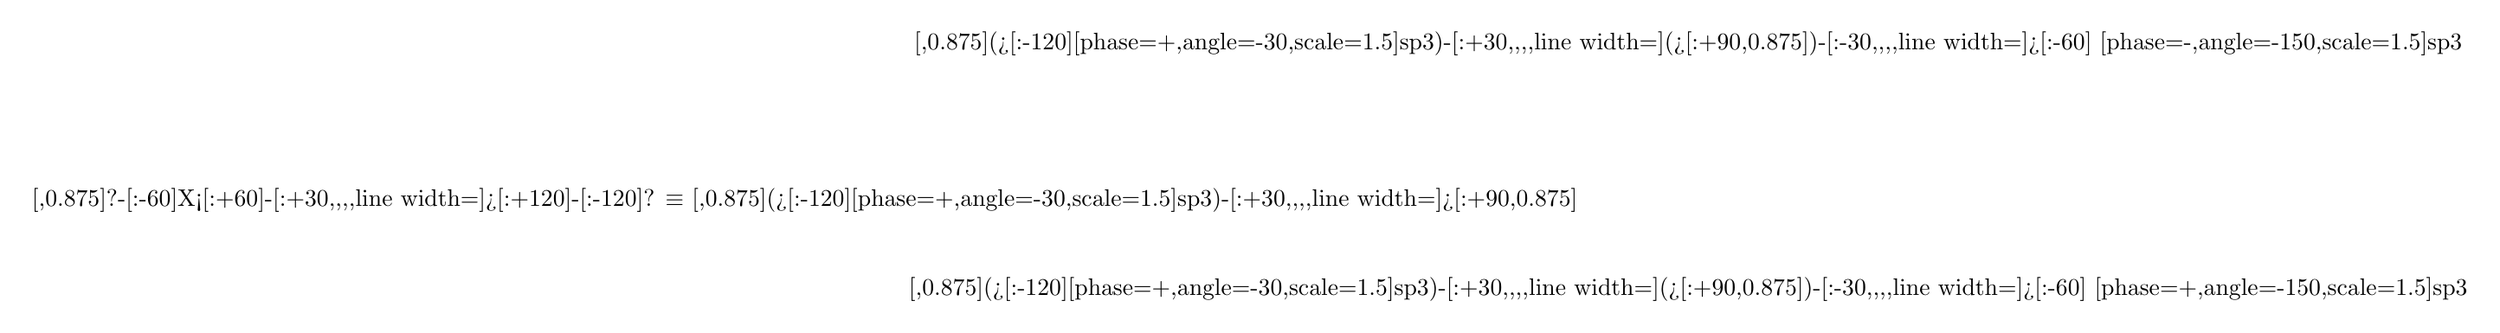
\begin{tikzpicture}[xscale=1.5]
  \begin{scope}[black,dashed]
\DrawTripleCorrelation{-0.5}{2.5}{-2.50}{-0.5}
\end{scope}
\begin{scope}[black,dotted]
\DrawTripleCorrelation{-0.5}{2.5}{ 1.50}{-0.5}
\end{scope}
  \draw(0.75,-0.5) node [anchor=east] {\chemfig[,0.875]{?-[:-60]X<[:+60]-[:+30,,,,line width=\boldbondwidth]>[:+120]-[:-120]?} $\equiv$ \chemfig[,0.875]{(>[:-120]\orbital[{phase=+,angle=-30,scale=1.5}]{sp3})-[:+30,,,,line width=\boldbondwidth]>[:+90,0.875]}};
  %\draw(4.25,-0.5) node [anchor=west] {\chemfig[,0.875]{(>[:-60]\orbital[{phase=+,angle=-150,scale=1.5}]{sp3})-[:+150,,,,line width=\boldbondwidth]>[:+90,0.875]} $\equiv$ \chemfig[,0.875]{?-[:-60]X<[:+60]-[:+150,,,,line width=\boldbondwidth]>[:+120]-[:-120]?}};
  \draw(1.75,-1.5) node [anchor=north] { \chemfig[,0.875]{(>[:-120]\orbital[{phase=+,angle=-30,scale=1.5}]{sp3})-[:+30,,,,line width=\boldbondwidth](>[:+90,0.875])-[:-30,,,,line width=\boldbondwidth]>[:-60]  \orbital[{phase=+,angle=-150,scale=1.5}]{sp3}}};
  \draw(1.75,1.5) node [anchor=south] { \chemfig[,0.875]{(>[:-120]\orbital[{phase=+,angle=-30,scale=1.5}]{sp3})-[:+30,,,,line width=\boldbondwidth](>[:+90,0.875])-[:-30,,,,line width=\boldbondwidth]>[:-60]  \orbital[{phase=-,angle=-150,scale=1.5}]{sp3}}};
\end{tikzpicture}

\vspace{5mm}
\end{figure}

\begin{figure}
\caption{Орбитальная диаграмма общего вида 3,7-взаимодействий%
%  неподелённых электронных пар в~конформации \CC{} аналогов бицикло[3.3.1]нонана
}\label{fig:Interactions:NonSym37}
  \centering

\vspace{5mm}
  \begin{tikzpicture}[xscale=1.5]
  \begin{scope}[black,dashed]
  \DrawTripleCorrelation{-0.75}{2.0}{-2.50}{-0.25}
  \end{scope}
  \begin{scope}[black,dotted]
  \DrawTripleCorrelation{-0.75}{3.0}{ 1.00}{-0.25}
  \end{scope}
  \draw(0.75, 0.25) node [anchor=east] {\chemfig[,0.875]{?-[:-60]X<[:+60]-[:+30,,,,line width=\boldbondwidth]>[:+120]-[:-120]?} $\equiv$ \chemfig[,0.875]{(>[:-120]\orbital[{phase=+,angle=-30,scale=1.5}]{sp3})-[:+30,,,,line width=\boldbondwidth]>[:+90,0.875]}};
  \draw(4.25,-1.0) node [anchor=west] {\chemfig[,0.875]{(>[:-60]\orbital[{phase=+,angle=-150,scale=1.5}]{sp3})-[:+150,,,,line width=\boldbondwidth]>[:+90,0.875]} $\equiv$ \chemfig[,0.875]{?-[:-60]Y<[:+60]-[:+150,,,,line width=\boldbondwidth]>[:+120]-[:-120]?}};
  \draw(1.0,-1.5) node [anchor=north] { \chemfig[,0.875]{(>[:-120]\orbital[{phase=+,angle=-30,scale=1.5}]{sp3})-[:+30,,,,line width=\boldbondwidth](>[:+90,0.875])-[:-30,,,,line width=\boldbondwidth]>[:-60]  \orbital[{phase=+,angle=-150,scale=1.5}]{sp3}}};
  \draw(3.5,1.5) node [anchor=south] { \chemfig[,0.875]{(>[:-120]\orbital[{phase=+,angle=-30,scale=1.5}]{sp3})-[:+30,,,,line width=\boldbondwidth](>[:+90,0.875])-[:-30,,,,line width=\boldbondwidth]>[:-60]  \orbital[{phase=-,angle=-150,scale=1.5}]{sp3}}};
\end{tikzpicture}

\vspace{5mm}
\end{figure}

При~взаимодействии подсистем $A$ и~$B$ парное возмущение молекулярных орбиталей $\phi_A$ и $\phi_B$ приводит к изменению их энергии, которое для низших порядках теории возмущения численно определяется из квадратного уравнения~\eqref{eq:Rauk:General:Perturbation}~\cite{Rauk:2001}

\begin{equation}\label{eq:Rauk:General:Perturbation}
\underbrace{\left[1-s^2_{AB}\right]}_{C_2}\cdot\epsilon^2 + \underbrace{\left[2s_{AB}h_{AB}+\epsilon_A+\epsilon_B\right]}_{C_1}\cdot\epsilon +\underbrace{\left[\epsilon_A\epsilon_B-h^2_{AB}\right]}_{C_0} = 0
\end{equation}
с дискриминантом $D=C_1^2-4 C_0 C_2$ и корнями $\epsilon_\pm = \frac{-C_1\pm\sqrt{D}}{2C_2}$, действительными при $D\ge 0$. Матричные элементы перекрывания $s_{AB}=\int d\tau\cdot\phi_A\phi_B$, одноэлектронного гамильтониана $h_{AB}=\int d\tau\cdot\phi_A\cdot\hat{h}\phi_B$

Дополнительным фактором, влияющим на относительные энергии конформеров \BC{}/\CB{} и~\CC{} являются взаимодействия положений 2 и~4 (6 и~8) внутри \tqt{крыльев}~(рис.~\ref{fig:Interactions:2468}). Они частично сходны с 1,3-диаксиальными взаимодействиями в соответствующих конформерах 1,3-\emph{цис}-дизамещённых аналогов циклогексана. Отталкивание приводит к уплощению циклов и сближению двух упомянутых форм.

\begin{figure}
  \caption{2,4~(6,8)-взаимодействия в молекулах аналогов бицикло[3.3.1]нонана}\label{fig:Interactions:2468}
  \centerfloat{}
\end{figure}

Примером полностью неорганической структуры с соответствующим скелетом является известный тетраборат-дианион \ce{H4B4O9^{2-}}~(\cmpd{Tetraborate}). В кристаллах, содержащих данный анион, \tqt{крылья} бициклической структуры планарны или незначительно скручены.
\begin{center}
  \begin{tabular}{ccc}
    \chemfig{HO-B*6(-O-B\rlap{${}^-$}(-[:-90]OH)(-[:0]O?)-O-B\rlap{${}^-$}(-[:+90]OH) (-[:0]O-[:-60]B?(-[:0]OH))-O-)} & \chemfig{R-B*6(--(-[:-90]R_1)(-[:0]?[a])--(-[:+90]R_2) (-[:0]-[:-60]?[a](-[:0]R_3))--)} & \\
    \cmpd{Tetraborate} & & \\
  \end{tabular}
\end{center}
3-борабицикло[$3.3.1$]нонаны (Бубнов, Лысенко).


Для незамещённого 3,7-дитиабицикло[3.3.1]нонана~\cmpd{Bicyclo331:37S2} расчётные данные предсказывают оптимальность формы~\BC{}.~\cite{Bushmarinov:2011,Pisarev:2013:rus,Pisarev:2013} Однако рентгеноструктурные данные свидетельствуют, что~скелет 1,5-ди\-метил-3,7-ди\-тиа\-би\-цик\-ло[3.3.1]но\-нан-9-се\-лона~\cmpd{Dithia37Selone9}~\cite{Brooks:1991} и~3,7-дитиа-1,5-ди\-аза\-би\-цик\-ло\-[$3.3.1$]\-но\-на\-на~\cmpd{Bicyclo331:37S2:15N2} принимает в кристаллической структуре конформацию \CC{}. Бициклические основы других 9-замещённых 1,5-ди\-метил-3,7-ди\-тиа\-би\-цик\-ло[3.3.1]но\-на\-нов "--- соединения~\cmpd{Dithia37NNPPh39}~\cite{Brooks:1993}, а также кетона~\cmpd{Dithia37Ketone9}~\cite{Brooks:1995} "--- обладают конформацией~\BC{}.

\begin{center}
  \begin{tabular}{cccc}
%\ChemPicture{S?[a]<[:-30,1.25]-[:+30,,,,line width=\boldbondwidth] (>[:+120]C(-[:+135,0.875]H)(-[:+45,0.875]H)-[:-120] (-[:-150]?[a]) (-[:-30]-[:-60]S?[b]))-[:-+30,,,,line width=\boldbondwidth]?[b,{<}]}~
\ChemPicture{S?[a]<[:-30,1.25]-[:+30,,,,line width=\boldbondwidth] (>[:+120]-[:-120] (-[:-150]?[a]) (-[:-30]-[:-60]S?[b]))-[:-+30,,,,line width=\boldbondwidth]?[b,{<}]} &
\ChemPicture{S?[a]<[:+60]-[:+30,,,,line width=\boldbondwidth](-[:+45,,,,line width=\boldbondwidth]CH_3)(>[:+120]C(=[:+90]Se)-[:-120] (-[:+135]H_3C)(-[:-150]?[a])(-[:-30]-[:-60]S?[b]))-[:-+30,,,,line width=\boldbondwidth]?[b,{<}]} &
\ChemPicture{S?[a]<[:+60]-[:+30,,,,line width=\boldbondwidth]N(>[:+120]-[:-120]N(-[:-150]?[a])(-[:-30]-[:-60]S?[b]))-[:-+30,,,,line width=\boldbondwidth]?[b,{<}]} &
\\
\cmpd{Bicycle331:37S2} &
\cmpd{Dithia37Selone9} &
\cmpd{Bicycle331:37S2:15N2} &
\\
\end{tabular}
~
\begin{tabular}{ccc}
\ChemPicture{S?[a]<[:-30,1.25]-[:+30,,,,line width=\boldbondwidth](-[:+60,,,,line width=\boldbondwidth]CH_3) (>[:+120]C(=[:+90,0.875]N-[:+30,0.75]NPPh_3)-[:-120] (-[:+120]H_3C) (-[:-150]?[a]) (-[:-30]-[:-60]S?[b]))-[:-+30,,,,line width=\boldbondwidth]?[b,{<}]} &
\ChemPicture{S?[a]<[:-30,1.25]-[:+30,,,,line width=\boldbondwidth](-[:+60,,,,line width=\boldbondwidth]CH_3) (>[:+120]C(=[:+90,0.875]O)-[:-120] (-[:+120]H_3C) (-[:-150]?[a]) (-[:-30]-[:-60]S?[b]))-[:-+30,,,,line width=\boldbondwidth]?[b,{<}]} &
\\
\cmpd{Dithia37NNPPh39} &
\cmpd{Dithia37Ketone9} &
\\
\end{tabular}
\end{center}

Бицикл [$3.3.1$] является составной частью множества каркасных структур. В~некоторых из~них сохраняется конформационная подвижность бицикла, в других конформации оказываются жёстко закреплены\dots

Скопин~\cmpd{Scopine} представляет собой 9-метил-3-окса-9-аза\-три\-цикло\-[$3.3.1.0^{2,4}$]\-нонан\-ол-7 и формально относится к семейству аналогов бицикло[$3.3.1$]нонана, хотя в первую очередь связан с алкалоидами ряда тропина~\cmpd{Tropine} (8-метил-8-азабицикло[$3.2.1$]октанола-3). Скелет~\cmpd{Scopine} находится в конформации \BC{}.~\cite{Ecija:2016}
Псевдопеллетьерин (9-метил-9-аза\-би\-цикло\-[3.3.1]нонан\-он-3)~\cmpd{Pseudopelletierine}
\cite{VallejoLopez:2017}, напротив, предпочитает \CC{}-формы [уточнить, которые именно!]

\begin{center}
\begin{tabular}{cc}
\ChemPicture{[:-30]N*6((-[:0,0.65]CH_3)>?[a]-[:-15]?[b]<O>(?[b])-[:-15](-[:180]-[:-120](<:[:180,0.75]HO)-[:-60]?[a])<)} & \\
\cmpd{Scopine} & \\
\end{tabular}
~
\begin{tabular}{cc}
\ChemPicture{HO>:*6(--(-[:+15]?[a])<N(-[:180,0.75]H_3C)>(-[:-15]?[a])--)} & \\
\cmpd{Tropine} & \\
\end{tabular}
~
\begin{tabular}{cc}
\ChemPicture{[:-30]N*6((-[:0,0.75]CH_3)-?----(-[:180]-[:-120]C(=[:180,0.875]O)-[:-60]?)-)} & \\ \cmpd{Pseudopelletierine} & \\
\end{tabular}

\end{center}

[3.3.1]-пропелланы "--- производные трицикло[$3.3.1.0^{1,5}$]нонана общей формулы~\cmpd{Propellanes331}.

\begin{center}
  \begin{tabular}{cc}
    %\ChemPicture{[:-30]Y*6(-?[a](-[:180]-[:120]X-[:+60]-[:0]?[a])--X---)}
    \chemfig{*5(--Y--(*5(--X--))(*3(-Z-))-)} ??? &  \\
    \cmpd{Propellanes331} & \\
  \end{tabular}
\end{center}

Карбопропелланы...

Скелет множества
3,7-дитиа-[$3.3.1$]-пропелланов~\cmpd{Propellanes331S37} (производные 3,7-дитиатрицикло$[3.3.1.0^{1,5}]$нонана) в~кристаллической фазе принимает конформацию \TT{} в достаточно широком ряду соединений: исходный~\cmpd{Propellanes331S37} и его комплексы с \ce{I2} и целым рядом хлоридов металлов. Молекулы дисульфоксида~\cmpd{Propellanes331SO37}, напротив, упаковываются в~кристаллах в форме \BC{}??? [смотрим внимательно!!!].~\cite{Herbstein:1986,Marsh:1988}


\begin{center}
  \begin{tabular}{ccc}
  \chemfig{*5(--S--(*5(--S--))(*3(--))-)} & \chemfig{*5(--S(=[:0]O)--(*5(--S(=[:180]O)--))(*3(--))-)} & \\
   \cmpd{Propellanes331S37} & \cmpd{Propellanes331SO37} & \\
\end{tabular}
\end{center}

Такое конформационное предпочтение трициклических систем, производных от~[$3.3.1$], вероятно, аналогично конформационному поведению шестичленного цикла в составе аналогов бицикло[$3.1.0$]гексана, в которых он обычно находится в форме \tqt{ванны}\dots

Тетрацикло[$3.3.1.0^{2,4}0^{6,8}$]нонаны~\cite{Bicker:1973}
\begin{center}
  \begin{tabular}{cc}\chemfig{[:-30]X*6(-(-[:180]?[c]-[:+120]?[a])-?[b]--?[b]-(-[:180]?[a]?[c])-)} & \\
  \end{tabular}
\end{center}

Триастеран...

\subsection{Биспидины (производные и гетероаналоги 3,7-диазабицикло[3.3.1]нонана)}

Катион протонированного 1,5-диметил-3,7-диазабицикло[3.3.1]нонан-9-она~\cmpd{BSP:O9:15Me2:HPlus} в кристаллах своих солей обнаруживает различную конформацию атома водорода связанного с нейтральным атомом азота в зависимости от способности аниона \ce{X-} к образованию водородных связей.

\begin{center}
  \begin{tabular}{ccc}
    \chemfig{N?[a](-[:-150]H)<[:+60]-[:+30,,,,line width=\boldbondwidth](-[:+45,,,,line width=\boldbondwidth]CH_3)(>[:+120]C(=[:+90,0.75]O)-[:-120] (-[:+135]H_3C) (-[:-150]?[a]) (-[:-30]-[:-60]N\rlap{${}^+$}?[b](-[:-135]H) (-[:-45]H)))-[:-+30,,,,line width=\boldbondwidth]?[b,{<}]} &
    \chemfig{N?[a](-[:-75]H)<[:+60]-[:+30,,,,line width=\boldbondwidth](-[:+45,,,,line width=\boldbondwidth]CH_3)(>[:+120]C(=[:+90,0.75]O)-[:-120] (-[:+135]H_3C) (-[:-150]?[a]) (-[:-30]-[:-60]N\rlap{${}^+$}?[b](-[:-105]H)(-[:-30]H)))-[:-+30,,,,line width=\boldbondwidth]?[b,{<}]} & \\
    \texttt{BOZGAA}~\cmpd{CCDC:BOZGAA} &
    \texttt{BOZFUT}~\cmpd{CCDC:BOZFUT} & \\
    (\ce{\cmpd{BSP:O9:15Me2:HPlus} + Cl^-.H2O}) & (\ce{\cmpd{BSP:O9:15Me2:HPlus} + CH3COO^-}) & \\
  \end{tabular}
\end{center}

9-окса-3,7-ди\-аза\-би\-цикло\-[3.3.1]\-нонаны~\cmpd{Bispidine:9O:RR}~\cite{Breuning:2009, Breuning:2011} и их комплексообразование c \ce{Pt(II)}~\cite{Pollak:2016}... 9-тиа-3,7-ди\-аза\-би\-цикло\-[3.3.1]\-нонаны~\cmpd{Bispidine:9S:RR}...


\begin{center}
  \begin{tabular}{ccc}
\ChemPicture{N?[a](-[:-150]R')<[:+60]-[:+30,,,,line width=\boldbondwidth](>[:+120]O-[:-120](-[:-150]?[a]) (-[:-30]-[:-60]N?[b](-[:-30]R'')))-[:-+30,,,,line width=\boldbondwidth]?[b,{<}]} &
\ChemPicture{N?[a](-[:-150]R')<[:+60]-[:+30,,,,line width=\boldbondwidth](>[:+120]S-[:-120](-[:-150]?[a]) (-[:-30]-[:-60]N?[b](-[:-30]R'')))-[:-+30,,,,line width=\boldbondwidth]?[b,{<}]} &
\\
\cmpd{Bispidine:9O:RR} &
\cmpd{Bispidine:9S:RR} &
\\
\end{tabular}
\end{center}
3,7-диметил-9,9-диоксо-9-тиа-3,7-ди\-аза\-би\-цик\-ло\-[3.3.1]\-но\-нан~\cmpd{Bispidine9SO2} по данным РСА находится в конформации~\CC{}. Структурные данные согласуются с результатами оптимизации соответствующей формы молекулы в приближении B3LYP / 6-31+G[dp].~\cite{Vlasova:2013:rus}
\begin{center}
\begin{tabular}{ccc}
\ChemPicture{N?[a](-[:-150]H_3C)<[:+60]-[:+30,,,,line width=\boldbondwidth](>[:+120]S(=[:+135,0.875]O)(=[:+45,0.875]O)-[:-120](-[:-150]?[a]) (-[:-30]-[:-60]N?[b](-[:-30]CH_3)))-[:-+30,,,,line width=\boldbondwidth]?[b,{<}]} &
\ChemPicture{N?[a](-[:-105]Tf)<[:+60]-[:+30,,,,line width=\boldbondwidth](>[:+120]N(-[:+90]Tf)-[:-120](-[:-150]?[a]) (-[:-30]-[:-60]N?[b](-[:-75]Tf)))-[:-+30,,,,line width=\boldbondwidth]?[b,{<}]} &
\\
\texttt{AFUFUE}~\cmpd{Bispidine9SO2}~\cite{Vlasova:2013} &
\texttt{TAYCUU}~\cmpd{Bispidine:9N:Tf3}~\cite{Shainyan:2017} & \\
\end{tabular}
\end{center}
Бициклический скелет \emph{трис}-трифторметилсульфонильного производного 3,7,9-три\-аза\-би\-цик\-ло\-[3.3.1]\-но\-на\-на~\cmpd{Bispidine:9N:Tf3}  согласно рентгеноструктурным данным~\cite{Shainyan:2017} также принимает конформацию \tqt{двойного кресла}~\CC{}.

%\section{Природные соединения, содержащие скелет бицикло[$3.3.1$]нонана}

\subsubsection{Хинолизидиновые алкалоиды}

Одним из представителей трициклических алкалоидов
является цитизин~\cmpd{Cytisine}. Родственные ему ромбифолин~\cmpd{Rhombifoline}. Тетрациклические: анагирин~\cmpd{Anagyrine}, термопсин~\cmpd{Thermopsine}, баптифолин~\cmpd{Baptifoline} и эпибаптифолин~\cmpd{Epibaptifoline}.~\cite{Goller:2019} 

\begin{center}
\begin{tabular}{ccc}
\chemfig{*6(-C(=[,0.75]O)-N(*6(--(-[:+30]-[:+90]NH-[:+150]?[a])<:>:?[a]-))-=-=)} & 
\chemfig{*6(-C(=[,0.75]O)-N(*6(--(-[:+30]-[:+90]N (-[:+30]-[:-30]-[:-90]=[:-150,0.75]H_2C)-[:+150]?[a])<:>:?[a]-))-=-=)} & \\
\cmpd{Cytisine} &
\cmpd{Rhombifoline} & 
\\
\end{tabular}
\end{center}

\begin{center}
\begin{tabular}{ccc}
    \chemfig{*6(-C(=[,0.75]O)-N(*6(--(-[:+30](*6(-----N)) (<:[:-90,0.75]H)-[:+90]\phantom{N}-[:+150]?[a])<>?[a]-))-=-=)} & 
    \chemfig{*6(-C(=[,0.75]O)-N(*6(--(-[:+30](*6(-----N)) (<[:-90,0.75]H)-[:+90]\phantom{N}-[:+150]?[a])<>?[a]-))-=-=)} & \\
\cmpd{Anagyrine} & \cmpd{Thermopsine} & \\
  \end{tabular}
\end{center}

\begin{center}
\begin{tabular}{ccc}
  \chemfig{*6(-C(=[,0.75]O)-N(*6(--(-[:+30](*6(--(<:[:-30,0.875]OH)---N)) (<:[:-90,0.75]H)-[:+90]\phantom{N}-[:+150]?[a])<>?[a]-))-=-=)} &
  \chemfig{*6(-C(=[,0.75]O)-N(*6(--(-[:+30](*6(--(<[:-30,0.875]OH)---N)) (<:[:-90,0.75]H)-[:+90]\phantom{N}-[:+150]?[a])<>?[a]-))-=-=)} & \\
  \cmpd{Baptifoline} & \cmpd{Epibaptifoline} & \\
  \end{tabular}
\end{center}

Пахикарпин или (-)-спартеин~\cmpd{Pachycarpine}, (+)-спартеин~\cmpd{Sparteine}.

\begin{center}
  \begin{tabular}{ccc}
    \chemfig{*6(--N(*6(--(-[:+30](*6(-----N)) (<:[:-90,0.75]H)-[:+90]\phantom{N}-[:+150]?[a])<>?[a]-))-(<[:+90,0.75]H)---)} & 
    \chemfig{*6(--N(*6(--(-[:+30](*6(-----N)) (<[:-90,0.75]H)-[:+90]\phantom{N}-[:+150]?[a])<:>:?[a]-))-(<:[:+90,0.75]H)---)} & \\
    \cmpd{Pachycarpine} & \cmpd{Sparteine} & \\
  \end{tabular}
\end{center}

Трициклический алкалоид ангустифолин~\cmpd{Angustifoline} по данным исследования ЯЭО и других экспериментов ЯМР представляет собой структуру с бициклом [$3.3.1$] в конформации~\CC{}, которая стабилизируется внутримолекулярным мостиком \ce{N\bond{...}H-N}.~\cite{Wysocka:1994} Аналогичная картина наблюдается в кристаллической структуре гидроиодида $\alpha$-изолупанина~\ce{{\cmpd{IsolupanineA}}.HI}~\cite{Koziol:1986}
 
\begin{center}
\begin{tabular}{ccc}
\chemfig{*6(-C(=[,0.75]O)-N(*6(--(-[:+30] (-[:-30]-[:+30,0.75]=[:+90,0.75]CH_2)
  (<:[:-90,0.75]H)-[:+90]NH-[:+150]?[a])<>?[a]-))-(<[:+90,0.75]H)---)} & 
\chemfig{*6(-C(=[,0.75]O)-N(*6(--(-[:+30] (*6(-----N))  (<[:-90,0.75]H)-[:+90]\phantom{N}-[:+150]?[a])<>?[a]-))-(<[:+90,0.75]H)---)} &
\\
\cmpd{Angustifoline} & \cmpd{IsolupanineA} &  \\
  \end{tabular}
\end{center}

\subsubsection{Изохинолиновые алкалоиды}

Производные морфинана содержат, как правило, фрагмент 2-азабицикло$[3.3.1]$нонана.

\subsubsection{Терпеноиды и терпеновые алкалоиды}

Структурное разнообразие изопреноидных метаболитов...

Ряд клована "--- карбобицикл.

Ряд пачуленола и другие. Конформационные затруднения.

Атидан~\cmpd{Atidane} и атизин~\cmpd{Atisine} "--- 3-азабицикло[3.3.1]нонан.  

%Атидан\index{атидан}~\cmpd{Atidane}
\begin{center}
  \chemfig{*6(-\chembelow{N}{H}--?[b] (-[:+90]-[:+150]?[a])-(<[:-60]-[:+20,,,,line width=\boldbondwidth]>[:-30](-[:-90]?[d])(-[:+30,1.5]-[:+0,1.125]?[c] (<[:-45,0.75]H)-[:+90]CH_3)-[:+120](?[b]) (-[:+90,0.75]H)<:[:-0]-[:-45,1.5]?[c](-[:+0,0.75]H)-[:-120]?[d])-(<[:+160,0.75]H) (-[:+90]?[a])-)}

\cmpd{Atidane}
\end{center}

Атизин\index{атизин}~\cmpd{Atisine}
\begin{center}
  \chemfig{*6(-N(*5(---O-))-(<:[:-90,0.75]H)-?[b] (-[:+90]-[:+150]?[a])-(<[:-60]-[:+20,,,,line width=\boldbondwidth]>[:-30](-[:-90]?[d]) (-[:+30,1.5](-[:+90]OH)(<[:-45,0.75]H)-[:+0,1.125]?[c]=[:+15]CH_2)-[:+120](?[b]) (-[:+90,0.75]H)<:[:-0]-[:-45,1.5]?[c](-[:+0,0.75]H)-[:-120]?[d])-(<[:+160]H_3C) (-[:+90]?[a])-)}

\cmpd{Atisine}
\end{center}?

Аконитановые алкалоиды, производные~\cmpd{Aconitane}, помимо системы 3-азабицикло[3.3.1]нонан, содержат ещё и карбобицикл; обе эти подструктуры не имеют общих атомов.

\begin{center}
  \chemfig{*6(-\chembelow{N}{H}-(<:[:-90,0.75]H)(*6(-?[c](<:[:-90,0.75]H)-(<[:-90,0.75]H) (*6(---(<[:+0,0.75]H) (-[:+120]?[b])--))-(<[:-30,0.75]H)-(<[:+90,0.75]H)(-[:+30]?[b])-))-(-[:+90]-[:+150]?[a])-(<[:-60]?[c,{<}])-(<[:+160,0.75]H) (-[:+90]?[a])-)}
  
  \cmpd{Aconitane}
\end{center}



\section*{*~*~*}

Таким образом, конформационное поведение производных и гетероаналогов бицикло[3.3.1]нонана в наибольшей степени определяется взаимопревращением тех конформеров, в которых бициклический скелет приобретает либо конформацию \CC{}, либо формы \BC{}/\CB{}.

Большинство современных физико-химических методов исследования структуры и~динамики молекул используют результаты неэмпирического моделирования строения по~крайней мере на этапе формирования структурных гипотез. Такая методология подразумевает выбор в пользу той или иной гипотезы, являющейся результатом математического моделирования \tqt{из~первых принципов}, на основании экспериментальных измерений.